% vim: set spell spelllang=es syntax=tex :

\section{Metodología experimental}

\label{metodologiaExperimental}

Para comprobar el funcionamiento del nuevo framework se grabo un vídeo a partir
del cual se crearon dos, uno con una resolución de 800x600 píxeles y otro con
una resolución de 1280x720 píxeles.

Se configuraron diferentes experimentos haciendo variar la cantidad de partes en
las que fueron divididos los cuadros entre 1 y 24, la cantidad de hilos de
ejecución para tareas de búsqueda entre 1 y 12, con ambos vídeos. Para comparar
los resultados de las diferentes configuraciones se midieron los \emph{FPS}
soportados por el sistema y el tiempo de espera máximo (obtenido a los
\emph{FPS} soportados por el sistema bajo la misma configuración).

Se configuraron diferentes experimentos haciendo variar la cantidad de partes en
las que fueron divididos los cuadros y la cantidad de hilos de búsqueda, para
ambos vídeos. Para comparar los resultados de las diferentes configuraciones se
midieron los \emph{FPS} soportados por el sistema y el tiempo de espera máximo
(obtenido a los \emph{FPS} soportados por el sistema bajo la misma
configuración).

Como la obtención del retardo máximo depende del conocimiento previo de los
\emph{FPS}, cada experimento se dividió en dos partes. En la primera parte se
busca la cantidad de \emph{FPS} soportados por el sistema para esa
configuración. Para esto, el programa procesa tantos cuadros del vídeo como
pueda en un cierto intervalo de tiempo. En la segunda parte se limita la
cantidad de cuadros por segundo (según el valor máximo de \emph{FPS} encontrado
en la primera parte del experimento) y se registra el tiempo de espera máximo.
Dado que se trata de un sistema de tiempo real, es importante determinar las
cotas inferiores del rendimiento. Por esto, se repitió cada experimento 10
veces, registrando sólo el peor valor obtenido para cada variable en cada
configuración.

Dada la gran cantidad de experimentos, se buscó el tiempo mínimo de ejecución
necesario para que éstos fueran representativos de una ejecución prolongada. Se
realizaron tres ejecuciones de 6 minutos cada una con una misma configuración:
11 hilos y 10 fragmentos procesando el vídeo de 800x600 píxeles de resolución.
El primer minuto no se contabilizó, con el fin de permitir que la ejecución se
estabilizara. Dado que los 6 minutos de vídeo no caben en la memoria RAM del
equipo de pruebas, el sistema fue modificado para reintroducir en la lista de
cuadros a procesar aquellos cuadros ya procesados. Los resultados se compararon
con ejecuciones utilizando la misma configuración, es decir: utilizando el mismo
framework modificado para reutilizar los cuadros, utilizando 11 hilos, y
dividiendo el vídeo de 800x600 píxeles de resolución en 10 fragmentos, pero
ejecutando de 11 a 20 segundos, y contabilizando sólo los últimos 10 segundos.
El uso del framework modificado para este experimento en particular tiene un
rendimiento menor al framework original, por lo que los resultados son distintos
a los presentados en la sección \ref{resultados} cuando se utiliza la misma
cantidad de fragmentos e hilos. En la tabla 1 se muestran los \emph{FPS}
obtenidos para cada ejecución. Se observa que las pruebas de 16 segundos son
representativas de ejecuciones más largas.

\begin{table}[h]
	\centering
	\begin{tabular}{c||c|c|c|c|c|c|c|c|c|c|c}

		Ejecución&6min&11s&12s&13s&14s&15s&16s&17s&18s&19s&20s\\

		\hline
		\hline

		1&166& 171& 170& 170& 170& 169& 166& 166& 166& 166& 165\\

		\hline

		2&166& 171& 170& 170& 170& 168& 167& 166& 166& 165& 166\\

		\hline

		3&166& 171& 170& 170& 170& 169& 166& 166& 167& 166& 165

	\end{tabular}

	\caption{Búsqueda de la duración mínima de los experimentos}

\label{tabla}

\end{table}

\section{Plataforma experimental}

\label{plataformaExperimental}

El equipo de pruebas cuenta un procesador Intel Xeon E5-2630. Éste es un
procesador de 6 núcleos con multithreading simultáneo de dos vías, una
frecuencia básica de CPU de 2,30GHz y 2,8GHz en modo turbo, 15MiB de memoria
caché L3, 256KiB de caché L2, 32Kib de caché L1 para datos, y 32 KiB de caché L1
para instrucciones. El equipo posee además 16GiB de memoria RAM. La jerarquía de
memoria se muestra en la figura \ref{topoMemoria}.

\begin{figure}[h]

	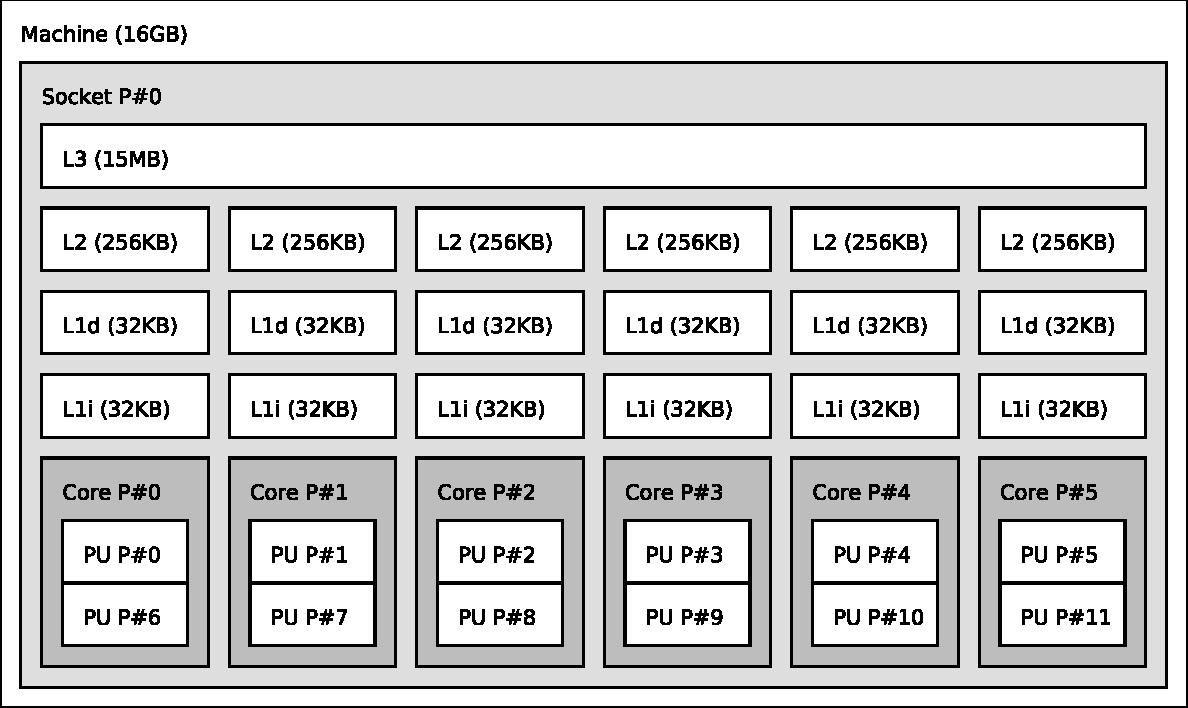
\includegraphics[width=\textwidth]{img/topo.pdf}
	\caption{Jerarquía de memoria de la máquina de pruebas.}

	\label{topoMemoria}

\end{figure}

\section{Diseño de experimentos y resultados}

\label{resultados}

Durante el desarrollo de la aplicación se probaron tres distintas
implementaciones. En la primera implementación, el framework ejecutaba las
distintas pilas de plugins en tareas separadas. En la segunda implementación el
framework fue modificado para que una sola tarea ejecutarán todas las pilas de
plugins sobre un mismo fragmento. Para la tercera implementación se trabajo
sobre el mismo framework que la segunda, pero se unieron las pilas de búsquedas
de robots y la de búsqueda de pelota. Para comprobar cual de éstas era la más
efectiva se realizaron las pruebas con cada una de éstas para la configuración
de 11 hilos de búsqueda y 10 fragmentos con el vídeo de 800x600 píxeles de
resolución. La primera implementación proceso 70 \emph{FPS}, la segunda 152
\emph{FPS} y la tercera 192 \emph{FPS}. Como esta última fue la que produjo
resultados más satisfactorios, sera sobre los resultados de ésta que
trabajaremos a continuación.

El sistema posee 6 núcleos con multithreading simultaneo de dos vías, por lo
cual como máximo puede ejecutar 12 hilos en paralelo. Por este motivo el rango
de la hilos de búsqueda sera inicialmente de 1 a 12 hilos, y en caso de que los
experimentos demuestren que el \emph{speedup} no ha comenzado a decaer, se
extenderá el rango hasta que esto suceda. El rango de cantidad de fragmentos
está limitado de 1 a 24.

En las figuras \ref{800fps} y \ref{1280fps} se muestran las cantidades de
\emph{FPS} alcanzados para un vídeo de 800x600 píxeles y 1280x720 píxeles
respectivamente, para distintas cantidades de hilos de búsqueda y fragmentos.
El número de hilos de búsqueda indica la cantidad de hilos que ejecutan las
tareas de búsqueda. Adicionalmente el sistema ejecuta dos hilos más para las
tareas estáticas, uno para la generación de cuadros y otro para la tarea de
generación de tareas de búsqueda. En el caso de del vídeo de 800x600 píxeles se
llego a un máximo de 196 \emph{FPS} cuando se divide el cuadro en 12 fragmentos
y se utilizan 5 hilos de búsqueda, mientras que para el vídeo de 1280x720
píxeles se alcanzo un máximo de 130 \emph{FPS} cuando se divide el cuadro en 24
fragmentos y se utilizan 10 hilos de búsqueda.

\begin{figure}[h]

	\includegraphics[width=\textwidth]{img/800x600_fps.pdf}
	\caption{FPS alcanzados por el sistema para vídeo de 800x600 píxeles}
	\label{800fps}

\end{figure}

\begin{figure}[h]

	\includegraphics[width=\textwidth]{img/1280x720_fps.pdf}
	\caption{FPS alcanzados por el sistema para vídeo de 1280x720 píxeles}
	\label{1280fps}

\end{figure}

En las figuras \ref{800fps} y \ref{1280fps} se pueden observar dos patrones que
ocurren en ambos vídeos. El primero es que si los cuadros se dividen en 7, 11,
17, 19 y 23 fragmentos, se produce una notable reducción en la cantidad de
cuadros por segundo con respecto a las divisiones adyacentes.

Esto se produce porque cuando los cuadros se dividen en un número primo de
fragmentos, el área total a procesar se incrementa de forma significativa con
respecto a los valores circundantes. En la figura \ref{primosArea} se muestra la
fluctuación de la suma del área de los fragmentos en divisiones de 1 hasta 100
fragmentos para un vídeo de 1280x720 píxeles de resolución, resaltando los
resultados para valores primos y para los valores inmediatamente inferiores y
superiores. Como puede observarse, a partir de 7 fragmentos el área total se
incrementa de forma significativa cuando el número es primo con respecto a los
valores cercanos con divisores. En estos casos, un incremento del número
de fragmentos aumenta el paralelismo, pero es acompañado de un incremento
drástico del área a procesar.

\begin{figure}[h]

	\includegraphics[width=\textwidth]{img/primos_area.pdf}
	\caption{Área total a procesar para número de fragmentos primos y sus inmediatos}
	\label{primosArea}

\end{figure}

Para comprobar como esta variación de volumen de datos afecta la cantidad de
cuadros por segundo procesados, se realizaron nuevas pruebas sobre el vídeo de
1280x720 píxeles de resolución, con 11 hilos de búsqueda y variando la cantidad
de fragmentos entre los números primos mayores a 24 y menores a 100, y sus
inmediatos superior e inferior. Los valores para números primos e inmediatos
inferiores a 24 fueron tomados de los experimentos anteriores. Los resultados
pueden ser observados en la figura \ref{primosFPS}.

\begin{figure}[h]

	\includegraphics[width=\textwidth]{img/primos_fps.pdf}
	\caption{FPS totales para número de fragmentos primos y sus inmediatos}
	\label{primosFPS}

\end{figure}

Como se puede observar en la figura \ref{primosFPS}, para una cantidad de
fragmentos menor a 7, el perjuicio por aumento en el área es menor que el
beneficio aportado por el incremento en el paralelismo. Para cantidades primas
de fragmentos menores a 7, la cantidad de FPS es inferior para la cantidad de
fragmentos inmediatamente anterior, y mayor para la cantidad de fragmentos
inmediatamente posterior. A partir de 7 fragmentos, se produce una reducción de
los FPS si la cantidad de fragmentos es un cantidad prima con respecto las
cantidades de fragmentos inmediatamente anterior y posterior. Si se observa la
figura \ref{primosArea}, dividir el cuadro en 7 fragmentos resulta en el primer
incremento notable de área con respecto tanto a un fragmento menos como un
fragmento más. También se pueden apreciar que los incrementos repentinos en el
área total coinciden con disminuciones repentinas en los cuadros por segundo
procesados.

El segundo patrón que se puede observar en las figuras \ref{800fps} y
\ref{1280fps} es que cuando la cantidad de fragmentos es baja y la cantidad de
hilos de búsqueda es alta, el sistema tiene menor \emph{FPS} que utilizar una
menor cantidad de hilos búsqueda pero una mayor cantidad de fragmentos. La
memoria caché se comparte entre los cuadros que están siendo procesados en
paralelo. Cuanto más cuadros se procesen en paralelo, mayor será la competencia
por la memoria caché. La cantidad de cuadros que se procesan en paralelo está en
relación con el número de fragmentos y la cantidad de hilos de búsqueda.
Considerando que la cantidad de hilos de búsqueda es mayor que la cantidad de
fragmentos, si se disminuye la cantidad de fragmentos, manteniendo la cantidad
de hilos de búsqueda, se incrementa la cantidad de cuadros a procesar en
paralelo. Esto tiene como efecto que los cuadros compitan por la caché y reduce
las posibilidades de que los fragmentos entren completamente en las cachés de
nivel más bajo. Por esto se propuso la hipótesis de que el retardo se produce
debido a un aumento en los fallos de caché.

Para comprobar que la hipótesis es correcta se diseñó el siguiente experimento.
Se ejecutó el programa procesando cuadros del vídeo de 1280x720 píxeles de
resolución, y se midieron los fallos de caché en configuraciones de 1, 2, 3, 4,
6 y 12 fragmentos y cantidad de hilos búsqueda de 1 a 11. Para obtener los
fallos de caché de nivel 3 (es decir, cuando es necesario acceder a datos en la
memoria RAM) se utilizó la herramienta \emph{perf}. Ésta es una aplicación que
permite acceder a los contadores de hardware del procesador que proveen datos
muy precisos con un overhead despreciable.

En la figura \ref{cacheFallos} se muestran los fallos de caché por cuadro
obtenidos en el experimento. En todas las curvas se produce un incremento
significativo de los fallos de cache cuando la cantidad de hilos de búsqueda se
aproxima al doble de la cantidad de fragmentos por cuadro\footnote{Cuando la
cantidad de hilos de búsqueda es el doble de la cantidad de fragmentos por
cuadro, la cantidad de fragmentos que se procesan concurrentemente es la
cantidad contenida en dos cuadros.}.

\begin{figure}[h]

	\includegraphics[width=\textwidth]{img/cache_fallos.pdf}
	\caption{Fallos de caché por cuadro para distintas cantidades de
	fragmentos}
	\label{cacheFallos}

\end{figure}

En las figuras \ref{800turnArround} y \ref{1280turnArround} se muestran los
tiempos máximos de espera de los cuadros, para los vídeos de 800x600 y 1280x720
píxeles de resolución (considerando que los \emph{FPS} son limitados al máximo
encontrado en la primera etapa de los experimentos).

\begin{figure}[h]

	\includegraphics[width=\textwidth]{img/800x600_turnArround.pdf}
	\caption{Tiempos máximos de espera en centésimas de segundo para el
	vídeo de 800x600 píxeles}
	\label{800turnArround}

\end{figure}


\begin{figure}[h]

	\includegraphics[width=\textwidth]{img/1280x720_turnArround.pdf}
	\caption{Tiempos máximos de espera en centésimas de segundo para el
	vídeo de 1280x720 píxeles}
	\label{1280turnArround}

\end{figure}

Estos dos últimas figuras nos permiten apreciar que no siempre una mayor
cantidad de cuadros por segundos procesados implicara el tiempo de espera
mínimo. Dependiendo de si se desea minimizar el tiempo de espera de los cuadros,
maximizar la cantidad de cuadros procesados, o encontrar un balance especifico,
se deberá elegir una cantidad de fragmentos y hilos de búsqueda apropiada. Por
ejemplo, en el caso del vídeo de 1280x720 píxeles de resolución, dividir la
imagen en 24 fragmentos y utilizar 10 hilos de búsqueda permite procesar 130
cuadros por segundo en el equipo de prueba, sin embargo el tiempo de espera es
de $0.28$ segundos. Si el cuadro se divide en 24 fragmentos y se utilizan 12
hilos de búsqueda, la cantidad de cuadros por segundo procesados cae a 128, pero
el tiempo de espera se reduce a $0.09$ segundos. Las figuras \ref{800tFPS} y
\ref{1280tFPS} sintetizan la relación entre los \emph{FPS} y el retardo de
cuadros, mostrando el mínimo retardo de cuadros para los diferentes \emph{FPS}
que puede alcanzar el sistema en cada vídeo.

\begin{figure}[h]

	\includegraphics[width=\textwidth]{img/800x600_tFPS.pdf}
	\caption{Tiempos máximos de espera para vídeo de 800x600 píxeles para
	los FPS soportados por el sistema}
	\label{800tFPS}

\end{figure}

\begin{figure}[h]

	\includegraphics[width=\textwidth]{img/1280x720_tFPS.pdf}
	\caption{Tiempos máximos de espera para vídeo de 1280x720 píxeles para
	los FPS soportados por el sistema}
	\label{1280tFPS}

\end{figure}

Las figuras \ref{bestFPS800} y \ref{bestFPS1280} muestran el máximo rendimiento
en cuadros por segundo obtenidos para cada configuración de hilos de búsqueda
incluyendo el retardo de cuadro, para los vídeos de 800x600 y 1280x720 píxeles.
Se puede apreciar en la figura que para el caso del vídeo de 800x600 píxeles el
sistema escala sólo hasta el uso de 5 hilos de búsqueda. En el caso del vídeo de
1280x720 píxeles, también muestra una reducción en el rendimiento cuando se
utilizan 12 hilos de búsqueda. Como la plataforma experimental puede ejecutar
hasta 12 hilos simultáneamente, los hilos de búsqueda deberán compartir recursos
con los hilos dedicados a las tareas estáticas. Por lo cual no podemos
determinar el punto en el cual la aplicación deja de escalar para un vídeo de
1280x720 píxeles, aunque se alcanza un punto de rendimientos decrecientes luego
de los 5 hilos de búsqueda.

\begin{figure}[h]

	\includegraphics[width=\textwidth]{img/800x600_bestfps.pdf}
	\caption{FPS máximos alcanzados para el vídeo de 800x600 píxeles para
	distintas configuraciones de cantidad de hilos de búsqueda. Se incluye
	el retardo de cuadro bajo la configuración y la cantidad de fragmentos
	en la que fue dividido.} \label{bestFPS800}

\end{figure}

\begin{figure}[h]

	\includegraphics[width=\textwidth]{img/1280x720_bestfps.pdf}
	\caption{FPS máximos alcanzados para el vídeo de 1280x720 píxeles para
	distintas configuraciones de cantidad de hilos de búsqueda. Se incluye
	el retardo de cuadro bajo la configuración y la cantidad de fragmentos
	en la que fue dividido.}
	\label{bestFPS1280}

\end{figure}

El \emph{speedup} del rendimiento (sobre los FPS) máximo alcanzado por el
sistema para el vídeo de 800$\times$600 píxeles es de $3.38\times$, mientras que
para el vídeo 1280$\times$720 es de $5.00\times$. Las curvas de \emph{speedup}
son mostradas en las figuras \ref{speedUp800} y \ref{speedUp1280}. Se puede
observar que en ambos casos el crecimiento es pronunciado hasta 5 hilos de
búsqueda, los cuales sumados a los hilos de ejecución para tareas estáticas
superan la cantidad de núcleos físicos de la plataforma experimental. Existen
dos posibles causas para la reducción del crecimiento del \emph{speedup}. La
primera es que con los cinco hilos de búsqueda más los dos hilos de ejecución
para tareas estáticas se logre suficiente paralelismo a nivel de instrucción,
alcanzando un alto uso de las unidades funcionales de cada núcleo. La segunda
posible causa del decremento del crecimiento del \emph{speedup} es que la
aplicación esté limitada por memoria, provocando que el acceso a los datos sea
cuello de botella, reduciendo el rendimiento cuando se utilizan más de seis
núcleos.

\begin{figure}[h]

	\includegraphics[width=\textwidth]{img/800x600_speedup.pdf}
	\caption{\emph{Speedup} para el vídeo de 800x600 píxeles}
	\label{speedUp800}

\end{figure}

\begin{figure}[h]

	\includegraphics[width=\textwidth]{img/1280x720_speedup.pdf}
	\caption{\emph{Speedup} para el vídeo de 1280$\times$720 píxeles}
	\label{speedUp1280}

\end{figure}
